% =================================================================
% Codice LaTeX PGFPlots NATIVO per i tre grafici del capitolo Risultati.
%
% Dati incinerati direttamente nel sorgente: niente file esterni.
% Pronto da incollare in Overleaf.
%
% Tre blocchi `figure` indipendenti + preambolo di pacchetti aggiuntivi.
% =================================================================


% =================================================================
% PREAMBOLO — aggiungere al preambolo del documento principale
% =================================================================
%
% \usepackage{pgfplots}
% \pgfplotsset{compat=1.18}
% \usepgfplotslibrary{fillbetween}
% \usetikzlibrary{patterns}
%
% (Non forziamo font: ereditato dal documento, p.es.\ Times via newtxtext.)
%
% =================================================================



% =================================================================
% FIGURA 1 — Robustezza di beta_str alla costruzione della componente di tasso
% =================================================================
%
% PROVENIENZA DATI:
%   - Baseline (proxy "Bordo 10Y via future"):
%       results/02_decomposition/baseline/decomp_canali.report.json
%       campi table_section_6_per_cell[*].{beta_str_central, sampling_band_low, sampling_band_high}
%       Run autoritativo del 2026-06-23T22:21:46Z (config_hash 907eb0ff..., seed
%       decomp_canali_2026-06-23). Le 4 celle robuste estratte:
%         NFP/neg   : beta_str = -1.4036, sampling band 95% = [-1.8929, -0.8879]
%         CPI/neg   : beta_str = +0.9509, sampling band 95% = [+0.5137, +1.4021]
%         FOMC/neg  : beta_str = +0.8748, sampling band 95% = [+0.3366, +1.4249]
%         CPI/pos   : beta_str = +2.2404, sampling band 95% = [+1.6022, +2.8560]
%
%   - Proxy alternative:
%       results/02_decomposition/true_curve_variants/results.json
%       campi results_per_variant[VAR][CELL].beta_str_central
%       VAR ∈ {C_baseline = "Tratto breve" (FFc3 puro),
%              B_multi    = "Multi-scad." (DGS 2-5-10 ponderate per D_n),
%              A_DGS10    = "Curva 10Y daily" (delta DGS10 daily)}
%
%       Valori (cella, C_baseline, B_multi, A_DGS10):
%         NFP/neg   : -0.8869, +0.1773, +0.2163
%         CPI/neg   : +0.7690, -0.0896, -0.0554
%         FOMC/neg  : +0.3654, -0.0429, -0.0081
%         CPI/pos   : +1.4506, -0.3918, -0.0502
%
\begin{figure}[t]
    \centering
    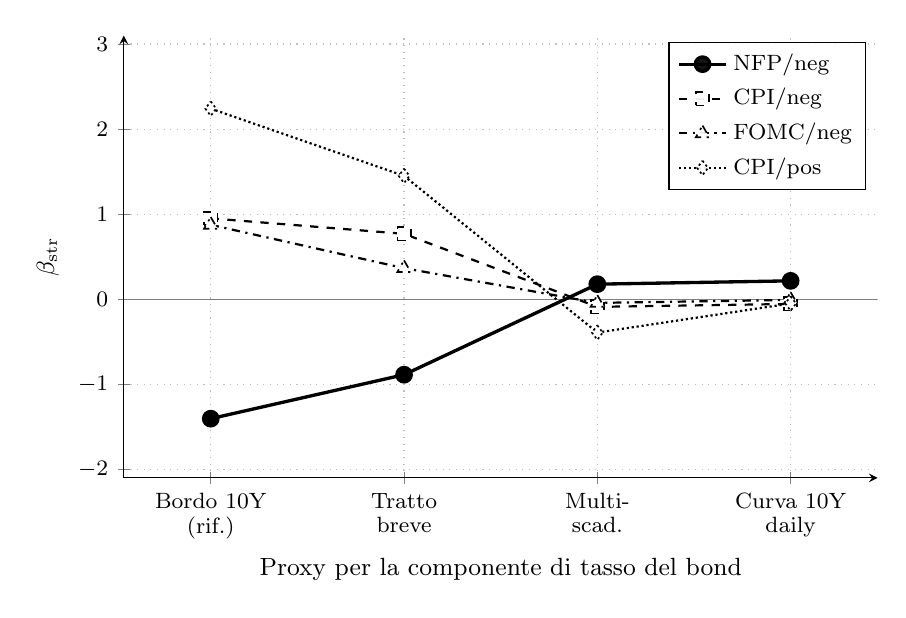
\begin{tikzpicture}
        \begin{axis}[
            width=0.92\linewidth,
            height=7.2cm,
            xtick={1,2,3,4},
            xticklabels={
                {\shortstack{Bordo 10Y\\(rif.)}},
                {\shortstack{Tratto\\breve}},
                {\shortstack{Multi-\\scad.}},
                {\shortstack{Curva 10Y\\daily}}
            },
            xticklabel style={font=\footnotesize, align=center},
            yticklabel style={font=\footnotesize},
            xlabel={Proxy per la componente di tasso del bond},
            ylabel={$\beta_{\mathrm{str}}$},
            xlabel style={font=\small},
            ylabel style={font=\small},
            xmin=0.55, xmax=4.45,
            ymin=-2.10, ymax=3.10,
            grid=both,
            major grid style={dotted, gray!50},
            minor grid style={dotted, gray!25},
            axis lines=left,
            legend cell align=left,
            legend style={
                at={(0.985, 0.985)}, anchor=north east,
                font=\footnotesize, draw=black, line width=0.4pt,
                fill=white, fill opacity=0.92, text opacity=1, row sep=1pt
            },
        ]

        % Linea y=0 (cambio segno)
        \draw[gray, thin] (axis cs:0.55,0) -- (axis cs:4.45,0);

        % NFP/neg (cella stabile, evidenziata)
        \addplot+[
            very thick, solid, black, mark=*, mark size=2.6pt,
            mark options={fill=black, draw=black},
            error bars/.cd, y dir=both, y explicit,
            error bar style={black, line width=0.8pt},
            error mark options={rotate=90, mark size=3.5pt, line width=0.7pt, black}
        ] table[row sep=\\] {
            x  y       y_low  y_high  \\
            1  -1.4036 0.4893 0.5157  \\
            2  -0.8869 0      0       \\
            3   0.1773 0      0       \\
            4   0.2163 0      0       \\
        };
        \addlegendentry{NFP/neg}

        % CPI/neg
        \addplot+[
            thick, dashed, black, mark=square*, mark size=2.4pt,
            mark options={fill=white, draw=black, line width=0.6pt},
        ] coordinates {(1,0.9509) (2,0.7690) (3,-0.0896) (4,-0.0554)};
        \addlegendentry{CPI/neg}

        % FOMC/neg
        \addplot+[
            thick, dashdotted, black, mark=triangle*, mark size=2.8pt,
            mark options={fill=white, draw=black, line width=0.6pt},
        ] coordinates {(1,0.8748) (2,0.3654) (3,-0.0429) (4,-0.0081)};
        \addlegendentry{FOMC/neg}

        % CPI/pos
        \addplot+[
            thick, densely dotted, black, mark=diamond*, mark size=2.6pt,
            mark options={fill=white, draw=black, line width=0.6pt},
        ] coordinates {(1,2.2404) (2,1.4506) (3,-0.3918) (4,-0.0502)};
        \addlegendentry{CPI/pos}

        \end{axis}
    \end{tikzpicture}
    \caption[Robustezza di $\beta_{\mathrm{str}}$ alla proxy della componente
             di tasso]{Coefficiente strutturale $\beta_{\mathrm{str}}$ per le
             quattro celle identificate dal cancello del pacchetto
             \texttt{decomposition}, al variare della proxy con cui si
             costruisce la componente di tasso $\Delta P^{B}_{b}$.
             Sull'asse $x$, in ordine: il bordo $10$Y del riferimento
             autoritativo (proxy $\Delta y_b = \Delta\,\mathrm{FFc3}$ con
             $D_{\mathrm{bond}}=8.97$); la stessa proxy del tratto breve in un
             secondo run di confronto; la combinazione multi-scadenza
             $2$--$5$--$10$ con pesi $D_n$; la curva $10$Y daily
             ($\Delta\,\mathrm{DGS10}$). La cella \texttt{NFP/neg} (cerchio
             pieno, linea continua spessa) conserva segno e magnitudine
             sotto le tre proxy intraday-coerenti; le altre tre celle
             attraversano lo zero sotto la proxy multi-scadenza o sotto la
             curva $10$Y daily. La barra di errore sul primo punto di
             \texttt{NFP/neg} \`e la banda di sampling al $95\%$ del bootstrap
             clusterizzato del baseline. La formulazione finale, in
             particolare le sfumature di onest\`a sulla robustezza
             condizionale alla scelta della proxy, \`e del committente.}
    \label{fig:robustezza_proxy}
\end{figure}



% =================================================================
% FIGURA 2 — Trasmissione del fattore QE lungo la curva Bund con banda 95%
% =================================================================
%
% PROVENIENZA DATI:
%   - results/05_ecb_curve_qe/results.json
%     campo results['step1_ecb_curve_symmetry']['results_per_maturity'] (LISTA, 15 elementi)
%     n_events = 129 (post-2010 con T/P/QE tutti disponibili)
%     n_qe_significant_BY = 12  (BY q=0.10, m=15, crit ~ 0.0241)
%
%   Tabella (mat, years, beta_QE, se_QE, by_rejected):
%     DE3M    0.25  -0.0557  0.0631  False
%     DE6M    0.50  -0.0468  0.0607  False
%     DE1Y    1.00  +0.1400  0.0662  False
%     DE2Y    2.00  +0.4001  0.0753  True
%     DE3Y    3.00  +0.5747  0.0704  True
%     DE4Y    4.00  +0.7412  0.0670  True
%     DE5Y    5.00  +0.8414  0.0902  True
%     DE6Y    6.00  +0.9502  0.0544  True
%     DE7Y    7.00  +0.9083  0.1041  True
%     DE8Y    8.00  +1.0734  0.0439  True
%     DE9Y    9.00  +1.1320  0.0498  True
%     DE10Y  10.00  +1.1430  0.0514  True
%     DE15Y  15.00  +1.1310  0.0727  True
%     DE20Y  20.00  +0.9737  0.0739  True
%     DE30Y  30.00  +1.0710  0.1228  True
%
%   Banda 95% = beta_QE +/- 1.96 * se_QE.
%   Asse x in scala radice quadrata: trasformo manualmente x -> sqrt(years), e
%   imposto i tick alla griglia naturale {0.25,1,2,5,10,15,20,30}.
%
\begin{figure}[t]
    \centering
    \begin{tikzpicture}
        \begin{axis}[
            width=0.95\linewidth,
            height=7.2cm,
            xmin=0.45, xmax=5.55,            % sqrt(0.20)=0.447, sqrt(31)=5.568
            ymin=-0.22, ymax=1.42,
            xtick={0.5, 1, 1.414, 2.236, 3.162, 3.873, 4.472, 5.477},  % sqrt(0.25,1,2,5,10,15,20,30)
            xticklabels={$0.25$, $1$, $2$, $5$, $10$, $15$, $20$, $30$},
            xticklabel style={font=\footnotesize},
            yticklabel style={font=\footnotesize},
            xlabel={Scadenza Bund (anni; scala radice)},
            ylabel={$\beta_{\mathrm{QE}}$},
            xlabel style={font=\small},
            ylabel style={font=\small},
            grid=major,
            major grid style={dotted, gray!50},
            axis lines=left,
            legend cell align=left,
            legend style={
                at={(0.985, 0.05)}, anchor=south east,
                font=\footnotesize, draw=black, line width=0.4pt,
                fill=white, fill opacity=0.95, text opacity=1, row sep=1pt
            },
        ]

        % Linea di riferimento y=1
        \draw[dashed, gray, thin] (axis cs:0.45,1) -- (axis cs:5.55,1);
        \draw[gray, thin]         (axis cs:0.45,0) -- (axis cs:5.55,0);

        % Banda 95%: upper e lower per fill_between
        \addplot [
            name path=upper, draw=none, forget plot
        ] table[row sep=\\] {
            x       y          \\
            0.5000  0.0680     \\  % sqrt(0.25); -0.0557+1.96*0.0631
            0.7071  0.0721     \\  % sqrt(0.5)
            1.0000  0.2697     \\
            1.4142  0.5477     \\
            1.7321  0.7127     \\
            2.0000  0.8725     \\
            2.2361  1.0182     \\
            2.4495  1.0568     \\
            2.6458  1.1123     \\
            2.8284  1.1594     \\
            3.0000  1.2296     \\
            3.1623  1.2437     \\
            3.8730  1.2734     \\
            4.4721  1.1185     \\
            5.4772  1.3117     \\
        };
        \addplot [
            name path=lower, draw=none, forget plot
        ] table[row sep=\\] {
            x       y          \\
            0.5000  -0.1794    \\  % -0.0557-1.96*0.0631
            0.7071  -0.1657    \\
            1.0000  0.0103     \\
            1.4142  0.2525     \\
            1.7321  0.4367     \\
            2.0000  0.6099     \\
            2.2361  0.6646     \\
            2.4495  0.8436     \\
            2.6458  0.7042     \\
            2.8284  0.9874     \\
            3.0000  1.0344     \\
            3.1623  1.0423     \\
            3.8730  0.9885     \\
            4.4721  0.8289     \\
            5.4772  0.8303     \\
        };
        \addplot [black!12] fill between [of=upper and lower];
        \addlegendimage{area legend, fill=black!12, draw=none}
        \addlegendentry{banda $95\%$ ($\pm 1.96\,\mathrm{SE}$)}

        % Linea centrale
        \addplot [
            black, thick, solid, forget plot
        ] table[row sep=\\] {
            x       y          \\
            0.5000  -0.0557    \\
            0.7071  -0.0468    \\
            1.0000  0.1400     \\
            1.4142  0.4001     \\
            1.7321  0.5747     \\
            2.0000  0.7412     \\
            2.2361  0.8414     \\
            2.4495  0.9502     \\
            2.6458  0.9083     \\
            2.8284  1.0734     \\
            3.0000  1.1320     \\
            3.1623  1.1430     \\
            3.8730  1.1310     \\
            4.4721  0.9737     \\
            5.4772  1.0710     \\
        };

        % Scadenze BY-rigettate (marker pieni neri)
        \addplot [
            only marks, mark=*, mark size=2.4pt,
            mark options={fill=black, draw=black}
        ] coordinates {
            (1.4142, 0.4001) (1.7321, 0.5747) (2.0000, 0.7412)
            (2.2361, 0.8414) (2.4495, 0.9502) (2.6458, 0.9083)
            (2.8284, 1.0734) (3.0000, 1.1320) (3.1623, 1.1430)
            (3.8730, 1.1310) (4.4721, 0.9737) (5.4772, 1.0710)
        };
        \addlegendentry{BY-rigettato ($q=0.10$)}

        % Scadenze non significative (marker vuoti)
        \addplot [
            only marks, mark=o, mark size=2.4pt,
            mark options={fill=white, draw=black, line width=0.7pt}
        ] coordinates {
            (0.5000, -0.0557) (0.7071, -0.0468) (1.0000, 0.1400)
        };
        \addlegendentry{non significativo}

        \end{axis}
    \end{tikzpicture}
    \caption[Trasmissione del fattore $\mathrm{QE}$ lungo la curva Bund]{
             Coefficiente $\beta_{\mathrm{QE}}$ della trasmissione del fattore
             $\mathrm{QE}$ di Altavilla et al.\ ($2019$) lungo la curva Bund a
             $15$ scadenze, dal $3$ mesi al $30$ anni. Linea nera continua:
             stima $\widehat{\beta}_{\mathrm{QE},n}$ per scadenza $n$; banda
             grigia: $\widehat\beta \pm 1.96\,\mathrm{SE}$ con errori standard
             $\mathrm{HC1}$. Marcatori pieni: scadenze che superano il
             controllo Benjamini--Yekutieli a $q=0.10$ con $m=15$ ipotesi
             ($12$ scadenze su $15$). Marcatori vuoti: scadenze non
             significative dopo correzione. Linea tratteggiata a $y=1$:
             livello di riferimento dell'unit\`a di trasmissione. Eventi
             $n=129$ (post-$2010$ con fattori $\mathrm{T/P/QE}$ tutti
             disponibili). Asse $x$ in scala radice quadrata per leggibilit\`a
             contemporanea del tratto corto e di quello lungo. La
             formulazione finale \`e del committente.}
    \label{fig:qe_bande}
\end{figure}



% =================================================================
% FIGURA 3 — Identificazione per eteroschedasticita' (NFP/neg)
% =================================================================
%
% PROVENIENZA DATI:
%   - Momenti per cella NFP/neg ricavati riassemblando i cluster del pacchetto
%     `protocol_v2` con stesso seed `execute_v2_signflip_2026-06-22`
%     (master_seed = 20260621, B_BOOT = 10000) sui dati Refinitiv intraday
%     (proprietary, fuori dalla repo pubblica).
%   - Compatibili con results/01_protocol_v2/beta_H_robust_cells_w15.json:
%     b_OLS = -0.7855, var_b_e = 757.4 bps^2, var_b_c = 49.2 bps^2,
%     r_hat = var_b_e / var_b_c = 15.39, cov_b_e = -5.95e-6 (= -594.9 bps^2),
%     cov_b_c = -2.29e-7 (= -22.87 bps^2), beta_H = ΔCov/ΔVar = -0.808
%     (SE_boot = 0.162, F_eff = 53.13). n_e = 145, n_c = 574.
%   - La varianza dell'equity non e' nel file di output del pacchetto 07; e'
%     stata estratta dalla matrice di covarianza 2x2 riassemblata in sessione,
%     conforme allo stesso protocollo:
%       var_e_event   = 1573.06 bps^2
%       var_e_control = 126.40  bps^2
%
%   Matrici di covarianza 2x2 in bps^2, base (bond=x, equity=y):
%     EVENTO    : [[757.40, -594.94], [-594.94, 1573.06]]
%     CONTROLLO : [[ 49.22,  -22.87], [ -22.87,  126.40]]
%
%   Decomposizione spettrale (chi^2_2(0.95) = 5.991):
%     EVENTO:
%       autovalori = 1886.54, 443.93
%       autovettore PC1 = (-0.4662, 0.8847) (sul piano (b,e))
%       angolo (deg) = 117.7847
%       semiasse maggiore a = sqrt(5.991*1886.54) = 106.31 bps
%       semiasse minore  b = sqrt(5.991* 443.93) =  51.57 bps
%     CONTROLLO:
%       autovalori = 132.66, 42.95
%       autovettore PC1 = (-0.2643, 0.9644)
%       angolo (deg) = 105.3246
%       semiasse maggiore a = sqrt(5.991*132.66) = 28.19 bps
%       semiasse minore  b = sqrt(5.991* 42.95) = 16.04 bps
%
%   Pendenze OLS (slope di rendimento equity su rendimento bond):
%     b_OLS_evento    = -0.7855  (= cov_e / var_b_e)
%     b_OLS_controllo = -0.4646  (= cov_c / var_b_c)
%
%   Stimatore strutturale beta_H = -0.808 e' Delta Cov / Delta Var, NON la
%   differenza di pendenze OLS: il grafico illustra il meccanismo (salto di
%   dispersione tra controllo ed evento), il valore strutturale si ottiene
%   dalla formula di Rigobon-Sack.
%
\begin{figure}[t]
    \centering
    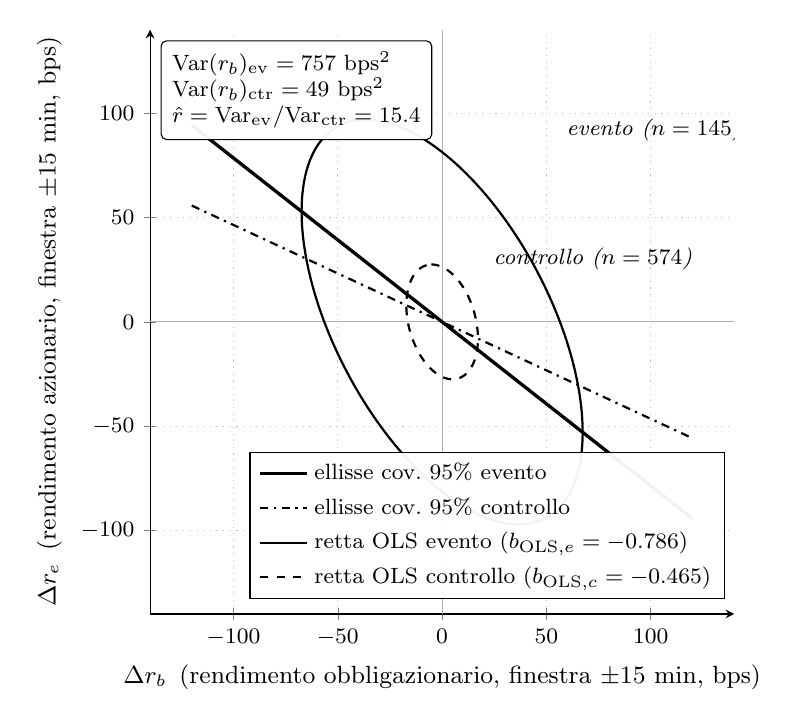
\begin{tikzpicture}
        \begin{axis}[
            width=0.82\linewidth,
            height=9.0cm,
            xmin=-140, xmax=140,
            ymin=-140, ymax=140,
            axis equal image,
            xlabel={$\Delta r_b$ \,(rendimento obbligazionario, finestra $\pm 15$ min, bps)},
            ylabel={$\Delta r_e$ \,(rendimento azionario, finestra $\pm 15$ min, bps)},
            xlabel style={font=\small},
            ylabel style={font=\small},
            xticklabel style={font=\footnotesize},
            yticklabel style={font=\footnotesize},
            xtick={-100,-50,0,50,100},
            ytick={-100,-50,0,50,100},
            grid=both,
            major grid style={dotted, gray!50},
            minor grid style={dotted, gray!25},
            axis lines=left,
            axis line style={black, thin},
            enlargelimits=false,
            clip=true,
            legend cell align=left,
            legend style={
                at={(0.985, 0.025)}, anchor=south east,
                font=\footnotesize, draw=black, line width=0.4pt,
                fill=white, fill opacity=0.95, text opacity=1, row sep=1pt
            },
        ]

        % Assi cartesiani (origine 0,0) sottili per riferimento visivo
        \draw[gray!60, thin] (axis cs:-140,0) -- (axis cs:140,0);
        \draw[gray!60, thin] (axis cs:0,-140) -- (axis cs:0,140);

        % Ellisse di covarianza 95% dell'EVENTO (chi^2_2(0.95)=5.991)
        % a = 106.31 (maggiore), b = 51.57 (minore), angolo = 117.78 deg
        \draw[black, thick, solid, rotate around={117.7847:(axis cs:0,0)}]
            (axis cs:0,0) ellipse [x radius=106.3120, y radius=51.5711];

        % Ellisse di covarianza 95% del CONTROLLO
        % a = 28.19, b = 16.04, angolo = 105.32 deg
        \draw[black, thick, dashed, rotate around={105.3246:(axis cs:0,0)}]
            (axis cs:0,0) ellipse [x radius=28.1921, y radius=16.0411];

        % Retta OLS evento (pendenza -0.7855)
        \addplot[
            black, very thick, solid, domain=-120:120, samples=2
        ] {-0.7855*x};

        % Retta OLS controllo (pendenza -0.4646)
        \addplot[
            black, thick, dashdotted, domain=-120:120, samples=2
        ] {-0.4646*x};

        % Etichette "evento" / "controllo" sulle ellissi
        \node[anchor=west, font=\footnotesize\itshape] at (axis cs:55,92)
            {evento ($n=145$)};
        \node[anchor=west, font=\footnotesize\itshape] at (axis cs:20,30)
            {controllo ($n=574$)};

        % Annotazione del salto di varianza (firma di Rigobon-Sack)
        % Posizionata in alto a sinistra fuori dalle ellissi
        \node[
            draw=black, line width=0.4pt, fill=white, fill opacity=0.95,
            text opacity=1, inner sep=4pt, rounded corners=2pt, font=\footnotesize,
            anchor=north west, align=left
        ] at (axis cs:-135,135)
            {%
                $\mathrm{Var}(r_b)_{\mathrm{ev}} = 757$ bps$^2$\\
                $\mathrm{Var}(r_b)_{\mathrm{ctr}} = 49$ bps$^2$\\
                $\hat r = \mathrm{Var}_{\mathrm{ev}}/\mathrm{Var}_{\mathrm{ctr}} = 15.4$
            };

        % Voci di legenda
        \addlegendimage{black, thick, solid}
        \addlegendentry{ellisse cov.\ $95\%$ evento}
        \addlegendimage{black, thick, dashed}
        \addlegendentry{ellisse cov.\ $95\%$ controllo}
        \addlegendimage{black, very thick, solid}
        \addlegendentry{retta OLS evento ($b_{\mathrm{OLS},e}=-0.786$)}
        \addlegendimage{black, thick, dashdotted}
        \addlegendentry{retta OLS controllo ($b_{\mathrm{OLS},c}=-0.465$)}

        \end{axis}
    \end{tikzpicture}
    \caption[Identificazione per eteroschedasticit\`a sulla cella
             \texttt{NFP/neg}]{Meccanismo dell'identificazione di Rigobon e
             Sack ($2003$, $2004$) sulla cella \texttt{NFP/neg}, finestra
             $\pm 15$ minuti, $n_e=145$ eventi e $n_c=574$ controlli. Le due
             ellissi rappresentano i contorni al $95\%$ delle distribuzioni
             $(\Delta r_b, \Delta r_e)$ nei due regimi, ottenute dagli
             autovalori delle matrici di covarianza $2{\times}2$. La
             differenza di dispersione del bond fra evento e controllo
             $\hat r = \mathrm{Var}(r_b)_{\mathrm{evento}}/\mathrm{Var}(r_b)_{\mathrm{controllo}} = 15.4$ \`e la
             firma dell'identificazione. Le rette $\mathrm{OLS}$ sui due
             regimi (pendenze $b_{\mathrm{OLS},e}=-0.786$ e
             $b_{\mathrm{OLS},c}=-0.465$) sono mostrate come illustrazione
             qualitativa del cambiamento di pendenza al passaggio
             controllo$\to$evento; lo stimatore strutturale di Rigobon e Sack
             \`e tuttavia
             $\widehat\beta_H = \Delta\,\mathrm{Cov}/\Delta\,\mathrm{Var} = -0.808$
             ($\mathrm{SE}_{\mathrm{boot}}=0.162$,
             $F_{\mathrm{eff}}=53.1$), \emph{non} la differenza
             $b_{\mathrm{OLS},e}-b_{\mathrm{OLS},c}$. La formulazione finale
             \`e del committente.}
    \label{fig:identificazione}
\end{figure}
